\newprob{1718701310}
{
    % act physcs p65 q2
    一個帶負電的小球以一根長 絲線懸起,當一個$\alpha$放射 源放在附近,小球的運動如 何?注意$\alpha$ 放射源能放出 正電荷,會擊走附近空氣粒 子的電子。
    \par{\par\centering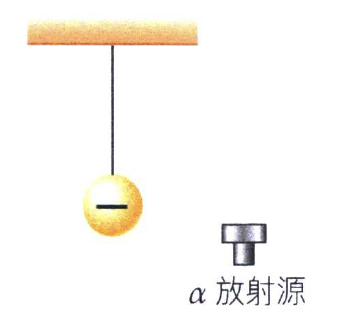
\includegraphics[width=.25\textwidth]{./img/ch1_electrostatics_lq_2024-06-18-17-03-33.png}\par}
    \begin{tasks}
        \task 小球向 $\alpha$ 放射源偏轉。
        \task 小球背向 $\alpha$ 放射源偏轉。
        \task 小球先向$\alpha$ 放射源偏轉,然後背向它偏轉。
        \task 小球停留在原來的位置。
    \end{tasks}
}{D}

\newprob{1718701450}
{
    % act physcs p65 q3
    三個金屬小球A、B和C完全相同。小球A 所帶 的電荷量為B的兩倍,彼此之間的電力為F。中 性的小球C先後觸碰A 和B。拿開小球C後,小 球A和B 之間的電力量值可能為多少?
    \begin{statements}
        \task 0
        \task $\dfrac{1}{2}F$
        \task $\dfrac{1}{4}F$
    \end{statements}
    \begin{tasks}(2)
        \task 只有(1)
        \task 只有(3)
        \task 只有(1)和(2)
        \task 只有(2)和(3)
    \end{tasks}
}{C}

\newprob{1718701603}
{
    % act physcs p65 q4
    一個小球$A$帶有  \qty{3}{\mu C} 的電荷,質量為  \qty{50}{g} ,以 絕緣輕繩懸起,輕繩可承受的最大張力為  \qty{10}{N} 。 另一個小球$B$帶有  \qty{-5}{\mu C} 的電荷,從小球$A$的正 下方慢慢地逼近。在繩子剛斷開前一刻,小球$B$ 相距小球 $A$ 多遠?
    \begin{tasks}
        \task  \qty{11.0}{cm}
        \task  \qty{11.3}{cm}
        \task  \qty{11.6}{cm}
        \task  \qty{11.9}{cm}
    \end{tasks}
}{D}

\newprob{1718701741}
{
    % act physcs p65 q5
    在正方形的四隻角上,擺放四顆帶有相同電荷量 值的粒子。以下哪些電荷分布能令置於正方形中 心的一顆粒子$X$處於平衡狀態?
    \begin{statements}(2)
        \task \topalign{\par\centering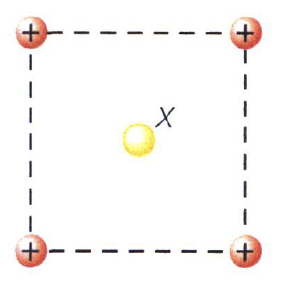
\includegraphics[width=.2\textwidth]{./img/ch1_electrostatics_mc_2024-06-18-17-09-42.png}\par}
        \task \topalign{\par\centering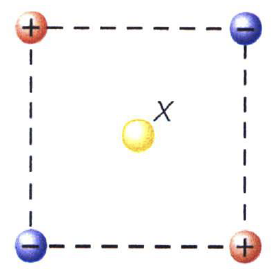
\includegraphics[width=.2\textwidth]{./img/ch1_electrostatics_mc_2024-06-18-17-09-50.png}\par}
        \task \topalign{\par\centering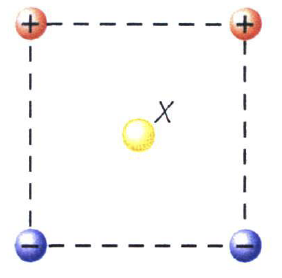
\includegraphics[width=.2\textwidth]{./img/ch1_electrostatics_mc_2024-06-18-17-09-58.png}\par}
    \end{statements}
    \begin{tasks}
        \task 只有(1)
        \task 只有(1)和(2)
        \task 只有(2)和(3)
        \task 由於粒子$X$上的電荷未明,因此無法判斷。
    \end{tasks}
}{B}

\newprob{1718701904}
{
    % act physcs p65 q6
    \textbf{(第5和6題)}現有兩顆固定的帶正電粒子$A$和 $B$,粒子$A$所載的電荷為$B$的兩倍。把另一顆帶 電粒子$P$放在$Y$點,其所受的淨電力為零。
    \par{\par\centering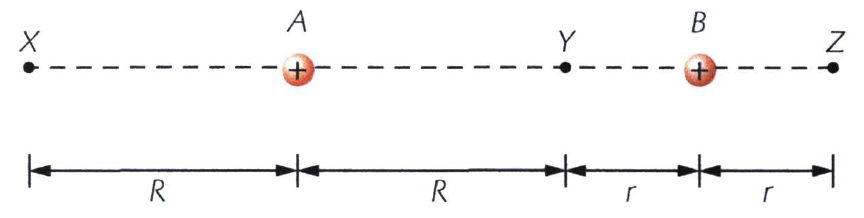
\includegraphics[width=.5\textwidth]{./img/ch1_electrostatics_mc_2024-06-18-17-12-00.png}\par}
    在下列各項敍述中,哪些是必定正確的?

    \begin{statements}
        \task $R$與$r$的比為 $\sqrt{2}:1$。
        \task $P$帶負電。
        \task 作用在$B$上的合電力沿着直線 $AB$。
    \end{statements}
    \begin{tasks}
        \task 只有(1)
        \task 只有(1)和(3)
        \task 只有(2)和(3)
        \task (1), (2) 和 (3)
    \end{tasks}
}{B}

\newprob{1718702093}
{
    % act physcs p65 q7
    下列哪一項關係式正確描述由電荷A和B 在不同 位置產生的合電場量值?
    \begin{tasks}
        \task $E_X>E_Z>E_Y>0$
        \task $E_X=E_Z>E_Y=0$
        \task $E_Z>E_X>E_Y=0$
        \task $E_Z>E_X>E_Y>0$
    \end{tasks}
}{C}

\newprob{1718702193}
{
    % act physcs p65 q9
    兩個帶電的金屬小球 $A$ 和$B$ 分別以兩條相 同長度的絕緣幼繩懸 起,圖示為兩個小球 靜止時的模樣。已知 小球 $A$ 的質量為$m$,試找出小球 $B$的質量
    \par{\par\centering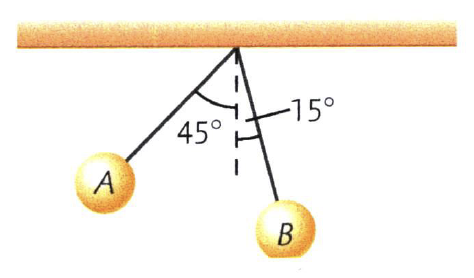
\includegraphics[width=.35\textwidth]{./img/ch1_electrostatics_mc_2024-06-18-17-17-19.png}\par}
    \begin{tasks}
        \task $1.37m$
        \task $2.73m$
        \task $3m$
        \task $3.73m$
    \end{tasks}

}{B}

\newprob{1718702294}
{
    % act physcs p65 q10
    一顆電子繞一顆原子核作圓周運動,半徑為$r$。若 角速度加倍,軌道的半徑現在應為多少?
    \begin{tasks}
        \task $\dfrac{1}{\sqrt[3]{4}}r$
        \task $\dfrac{1}{2}r$
        \task $2r$
        \task $\sqrt[3]{4}r$
    \end{tasks}

}{A}

\newprob{1718702469}
{
    % act physcs p65 q11
    在下列各項關於電場線的敍述中,哪些\textbf{必定}是正 確的?
    \begin{statements}
        \task 電場線不會接觸對方。
        \task 電場強度沿電場線方向增加。
        \task 在電場線上,作用在任何一顆點電荷上的電 力都是沿着電場線的切線方向。
    \end{statements}
    \begin{tasks}
        \task 只有(1)
        \task 只有(3)
        \task 只有(1)和(3)
        \task 只有(2)和(3)
    \end{tasks}

}{A}

\newprob{1718702528}
{
    % act physcs p65 q12
    一對垂直的平行金屬板分別連接至超高壓電源的 正極和負極。當一片帶電的鋁箔條置於兩板之 間,鋁箔條便會偏轉,如圖。
    \par{\par\centering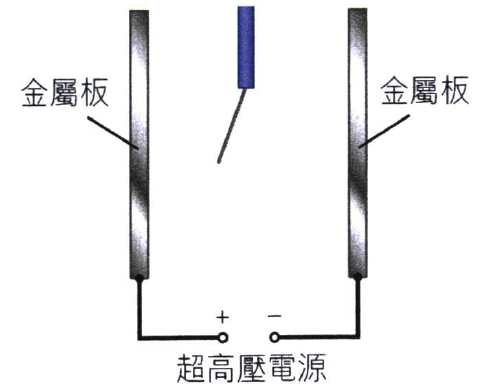
\includegraphics[width=.35\textwidth]{./img/ch1_electrostatics_mc_2024-06-18-17-22-18.png}\par}
    下列哪一個方法能增加鋁箔條偏轉的程度?
    \begin{statements}
        \task 增加超高壓電源的輸出電壓。
        \task 進一步分開兩塊板。
        \task 把鋁箔條移向負電板。
    \end{statements}
    \begin{tasks}
        \task 只有(1)
        \task 只有(2)
        \task 只有(2)和(3)
        \task (1), (2) 和 (3)
    \end{tasks}
}{A}

\newprob{1718702589}
{
    % act physcs p65 q13
    在一個水平的勻強電場中,一顆點電荷如圖示般 從A 點移至B點。假如點電荷只受到電力作用, 下列哪些敍述是正確的?
    \par{\par\centering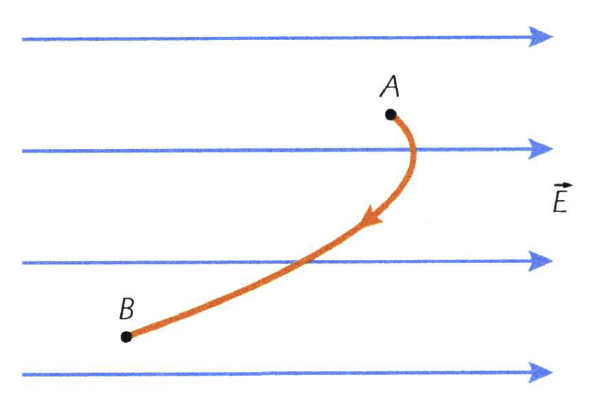
\includegraphics[width=.35\textwidth]{./img/ch1_electrostatics_mc_2024-06-18-17-23-24.png}\par}
    \begin{statements}
        \task 點電荷帶負電。
        \task 點電荷的加速度減少。
        \task 點電荷的垂直速度增加。
    \end{statements}
    \begin{tasks}
        \task 只有(1)
        \task 只有(1)和(3)
        \task 只有(2)和(3)
        \task (1), (2) 和 (3)
    \end{tasks}
}{A}